%
%
% this has already been updated, e.g. by considering the following (and other) questions:
% https://myuni-canvas.adelaide.edu.au/courses/25369/discussion_topics/106176
% https://myuni-canvas.adelaide.edu.au/courses/25369/discussion_topics/103778
%
%
%


\documentclass{pracs}
\usepackage{cases}
\newcommand{\duedate}{29 March 2019}
\newcommand{\longname}{Assignment 1}
\newcommand{\pracname}{prac1}
\newcommand{\ignore}[1]{}
\newtheorem{exercise}{Exercise}
\begin{document}
\title{Assignment 1: Basics and Testing}
\maketitle
\thispagestyle{fancy}

%\commonintro

	Formative, 	Learning objectives (1,2,3),\\
 	Abstraction (4), 	Design (4), 	Communication (4), 	Data (5),	Programming (5)

%\textbf{In addition}, submit your source code for Exercises $2$ and $3$ using the students forum at %\begin{verbatim} http://forums.cs.adelaide.edu.au/course/view.php?id=340 \end{verbatim}



\noindent 

 \begin{center}
    Due date: 11:59pm, \duedate, Weight: 5.0 \% of the course
  \end{center}




\section{Overview}
THIS assignment need to be done \emph{individually}. 
% in groups consisting of four (4) students.  If you have problems finding a group partner use the forum to search for group partners or contact the lecturer.

\textbf{Reminder:} unless we explicitly allow it for specific exercises, you must not copy and paste from websites, scientific articles, your friends, ...

\textbf{For this assignment you will have to hand in a report with the answers to the questions, and describing what you have done. In case you decide to write your own code,  you will need to include the code in your submission.}

%For consulting please contact Markus Wagner at markus@cs.adelaide.edu.au.

%\textbf{Each assignment has to be handed in and reasonable effort has to be made to complete each assignment in order to pass the course.} 

\section{Assignment}


\ignore{\begin{exercise}
Team work: who has done what? (zero points)
\end{exercise}
We'd like each team member to write one paragraph about what he or she has contributed to this assignment. We will not mark this, and it will not have any effect on the marking of the other exercises. You might now ask "why do this then?" --- well, through this no-stakes approach, we'd like to encourage self-regulation within the group and cooperative learning. You can't lose, you can only win.
}
%%%%%%%%%%%%%%%%%%%%%%%%%%%%%%%%%%%%%%%%%


\begin{exercise}
SBSE problems, our choice (8 points)
\end{exercise}

Software development effort estimation is the process of predicting the most realistic amount of effort (expressed in terms of person-hours or money or software size) required to develop or maintain software based on incomplete, uncertain and noisy input. 

The problem:\\
You are given a set of $n$ well-formed equations (i.e., $E_1$, $E_2$, $E_3$, \ldots, $E_n$) that can be used to produce cost predictions and a set of real-world data. From these, you need to select the equation $E_i$ with the best predictive capability.

Answer the following questions:
\begin{enumerate}
\item What are the objectives?
\item How can an example solution look like, i.e., what is the problem representation?
\item How would you measure the fitness of a solution for a single objective?
\item Which search algorithm would you choose? Why?
\end{enumerate}

In your report, be comprehensive in your answers. 

\begin{exercise}
SBSE problems, your choices (32 points)
\end{exercise}

Describe four (4) other software engineering problems (different from the one in Exercise 1) to which SBSE techniques can be applied to. 

In all four cases:
\begin{enumerate}
\item describe the problem, 
\item describe why it is fit for SBSE (hint: think about the search space), 
\item describe a possible problem representation (including how you would create neighbouring solutions), and 
\item propose a fitness function.
\end{enumerate}


Notes:
\begin{itemize}
\item In your report, be comprehensive in your answers. Think of a real-world situation where Mahmoud (who will mark your assignment) is your team leader who needs to be convinced.
\item The problems can be (but don't have to be) from the papers that you will be presenting and discussing in the spotlight talks and essays. This is to encourage you to start early with your spotlight talks and essays :) If you decide to go with this option, then please provide the URL to the paper.
\item Remember that fundamental combinatorial problems, such as travel salesman and knapsack problems, are not SBSE problems.  
\end{itemize}


\begin{exercise}
Artificial interaction testing  (20 points)
\end{exercise}

\textbf{Part 1}

Look up "combinatorial interaction testing". Provide a definition and a brief (but complete) example.

You can use online resources, such as Wikipedia, without losing points. However, it is mandatory that you properly reference the resource. For more information on proper referencing, see \url{https://www.adelaide.edu.au/writingcentre/resources/referencing-guides}. For this assignment, you can use, for example, the Harvard style. % and\\ \url{https://www.adelaide.edu.au/writingcentre/docs/harvard-style-guide.pdf}.

\textbf{Part 2}

Given is a Car Model, where car configurations can be customised by selecting components from options. Generate a comprehensive 4-way interaction test suite, which consists of as many valid tests as possible, for the following set of configurations for the following Car Model:

\begin{itemize}
\item Automated Driving Controller: included, none
\item Collision Avoidance Braking: StandardAvoidance, EnhancedAvoidance
\item Parallel Parking: included, none
\item Lateral Range Finder: included, none
\end{itemize}

It is important that your test suite respects our following constraints:
\begin{itemize}
\item Parallel parking must always be included.
\item If automated driving controller is included, then collision avoidance braking must be enhanced.
\item If collision avoidance braking is enhanced, then lateral range finder must be included.
\end{itemize}

Inn your report, include a description of how you generated the tests and how you considered the constraints. This description should be no longer than two pages.

Note: You can see this as a scenario from Software Product Line Engineering (SPLE), and your task is to find the valid combinations. In SPLE, the goal is to create collections of similar products from a shared set of assets. Here is a visualisation of the overall situation, created in Eclipse:

\begin{center}
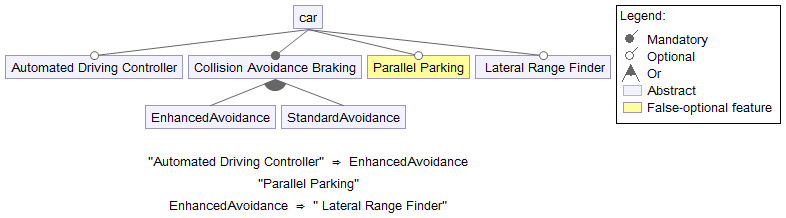
\includegraphics[width=130mm]{q3p2_car_assignment1AbstractConstraints.png}
\end{center}

False-optional feature means that it is declared optional, but it is always selected if its parent (car) is selected.


\begin{exercise}
Real-world interaction testing (40 points)
\end{exercise}

\textbf{Part 1}

Look up "pairwise testing". Provide a definition and a brief (but complete) example.

Your example needs to be different from the one you are submitting as an answer for Exercise 3.

You can use online resources as stated in Exercise 3, if you following our referencing requirement.

As before, be comprehensive in your answers. Think of a real-world situation where Mahmoud (who will mark your assignment) is your team leader who needs to be convinced.

\textbf{Part 2}

Django is a very popular Python-based framework for rapid development of web-based applications. Among popular sites using it are: Instagram, Mozilla and The Washington Times. Django is written in Python and comes with a global settings file that contains parameters that can be configured in any Django-based web application. 

Given the settings file at \url{https://github.com/django/django/blob/master/django/conf/global_settings.py}, answer the following questions:

\begin{enumerate}
\item How many parameters are there in the Django settings file?
\item List all the Boolean parameters.
\item Create a pairwise test suite for all Boolean parameters, and describe how you have done this. Aim at creating a minimal pairwise test suite. 
\end{enumerate}

Notes:
\begin{itemize}
\item You are not allowed to use any existing software for the generation of the test suite.
\item Provide the list of tests as an additional plain text file (no PDF/DOCX/...). In this file, list one test case per line, in any human-readable encoding you like.
\item It is NOT necessary to provide executable code that runs Django.
\end{itemize}







\section{General procedure for handing in the assignment}
Work should be handed in using the course website. The submission should include:
\begin{itemize}
\item pdf file of your solutions for theoretical assignments
\item all source files (if you created any)
\item descriptions as required in the statement of the exercises
\item a file name README.txt that contains instructions to run the code (if any), the names, student numbers, and email addresses of the group members
\end{itemize}

Note: as there is little to no coding involved in this assignment, there will be NO progress presentation session for this assignment.

%In addition, there will be a progress discussion session where you will have to explain your solutions:
%
%\begin{enumerate}
%\item All groups need to explain their solutions to parts of exercises in the assignment.
%\item Each member of a group shall be able to explain their solution. An answer like "my group partner did this, hence I can't explain this solution" will be counted as "no explanation" ($\rightarrow$ 0 marks for the particular part).
%\item Absence without a formal excuse\footnote{Markus Wagner and Junhua Wu need to be informed via email \emph{before} the discussion session.} for the session will be counted as "no explanation" if the person is chosen to explain his/her solution.
%\end{enumerate}

\end{document}
